%%% File encoding: UTF-8
%% äöüÄÖÜß  <-- no German Umlauts here? Use an UTF-8 compatible editor!

%%% Magic comments for setting the correct parameters in compatible IDEs
% !TeX encoding = utf8
% !TeX program = pdflatex 
% !TeX spellcheck = en_US
% !BIB program = biber

\documentclass[master,english]{hgbthesis}
% Permissible options in [..]: 
%   Type of work: diploma, master (default), bachelor, internship 
%   Main language: german, english (default)
%%%--------------------------------------------------

\RequirePackage[utf8]{inputenc}		% Remove when using lualatex or xelatex entfernen!

\graphicspath{{images/}}    % location of images and graphics
\logofile{logo}				% logo file = images/logo.pdf (use \logofile{} for no logo)
\bibliography{references}  	% name of bibliography file (references.bib)

%%%--------------------------------------------------
% Title page entries
%%%--------------------------------------------------

%%% Entries for ALL types of work: ------------------
\title{Pedestrian Warning System}
\author{Tobias Zuber}
\programname{Mobile Computing}
\placeofstudy{Hagenberg}
\dateofsubmission{2018}{09}{03}	% {YYYY}{MM}{DD}

%%% Restricted publication license instead of CC 
%   (master only):
% \strictlicense

%%%--------------------------------------------------
\begin{document}
%%%--------------------------------------------------

%%%--------------------------------------------------
\frontmatter		% title part (roman page numbers)
%%%--------------------------------------------------

\maketitle
\tableofcontents

\chapter{Abstract}

In recent years the trend of automation gained an increase in our society and sparked, in the field of the automotive automotive industry, to the existence of assisted driving technologies and self-driving vehicles. With this development the awareness and precaution towards participating parties must be taken in consideration as well.

To achieve this the goal of this thesis is the introduction and development of a \textit{Pedestrian warning System} prototype, which offers the recognition of nearby pedestrians, using the location information of nowadays commonly carried mobiles devices (e.g. smartphones), which will be forwarded to road-side units (RSU). These RSU are placed next to roads and allow the Evaluation of received locations and the transmission of a \textit{Pedestrian warning} to possibly endangered vehicles using vehicle-to-everything (V2X) communication.

% This should be a 1-page (maximum) summary of your work in English.


\chapter{Kurzfassung}

\begin{german}
In vergangen Jahre etablierte sich die Automatisierung als ein wachsender Trend und rief, insbesondere im Bereich der Automobilindustrie, die Entwicklung von Fahrassistenz-Systemen und selbstfahrenden Fahrzeugen hervor. Einhergehend mit der Entwicklung solcher Lösungen muss auch das Bewusstsein und die Vorsicht gegenüber den beteiligten Verkehrsteilnehmer berücksichtigt werden.

Daher ist es das Ziel dieser Thesis ein Prototyp eines \textit{``Fußgänger-Warnsystems''} zu entwickeln, welches die Erkennung von in der Nähe befindlichen Fußgängern ermöglicht und an die straßenseitigen Infrastruktur (RSU) weiterleitet.
Bei Empfang der Standortinformation wertet die RSU die einzelnen Standorte aus und verschickt, sofern Gefahr für ein Fahrzeug besteht, eine ``Fußgänger-Warnung'' mittels dem Vehicle-to-everything (V2X) Kommunikationsstandard an das betroffene Fahrzeug.

\end{german}

%%%--------------------------------------------------
\mainmatter         % main part (arabic page numbers)
%%%--------------------------------------------------

\chapter{Introduction}
\label{cha:Introduction}

\section{Motivation}
Vehicular transportation is an integral part of our everyday lives. Since the invention of the automobile in [x], vehicles aid people by covering (far) distances in a quick timely manner, while offering the availability to transport goods as well. Due to the versatility and increasing affordability of vehicles, the road infrastructure made available becomes increasingly busy, unclear and insecure - for all its participants. This phenomena is especially visible, but not limited to, urban areas. Roads are not exclusively in use by vehicles, but shared with other traffic participants such as pedestrians, cyclists, etc. Even with already existing controlling prerequisites, like traffic rules, signs and lights, a certain danger still persists. Traffic participants hidden from view, inattentive or distracted cause an endangerment for others and themselves. 

Participants most risk are pedestrians
% https://www.ncbi.nlm.nih.gov/pubmed/26547018
as they have the least accident protection compared to the safety measures in vehicles.
% statistics on accidents, share of pedestrian and cyclists
According to the European Commission Report ''Road Safety in the European Union'' 21\% of people killed on roads are pedestrians. The report points out that particularly urban areas expose the most danger towards vulnerable road users \cite{EURoadSafetyReport2017}.
Further, the World Health Organization (WHO) states that road traffic injuries are currently estimated to be the ninth leading cause of death globally and predicts to become the seventh leading cause by 2030 \cite{WHOGlobalReportRoadSafety}.

% idea why 
In order to decrease this inflicted endangerment towards pedestrians by vehicles sharing the road and increase their safety this thesis' aim is to introduce a ``Pedestrian warning system''. The systems goal is to notify vehicles about pedestrians in the proximate area who could be a potential endangerment. Having this information would then allow for imminent correction of maneuvering, routing and acceleration to circumvent collisions.

% prospect to the future; more cars as well as more pedestrians
A system like this needed as it is expected that the number of vehicles, traffic participants on roads increases even more \cite{}, but also as it is the foundation and requirement for autonomous driving in the future.  Having such a system in place is additionally beneficial since it aids the public's peace of mind and helps overcome possible trust issues towards the trend of autonomous vehicles.

The applied technology in the proposed ``Pedestrian Warning System'' is vehicle-to-everything (V2X) communication, which is the passing of information from a vehicle to any entity that may affect the vehicle, and vice versa. Such entities include, but are not limited to vehicles, infrastructure and pedestrians. V2X is already incorporated in newer vehicles of the upper mid range to luxury price range.
A pledge has also been made by the most important automobile manufacturers (Audi, Daimler, Ford, etc.)
% src = https://blog.nxp.com/automotive/v2x-is-ready-to-go; https://www.car-2-car.org/fileadmin/downloads/PDFs/170815_C2C_General_Flyer_Screen.pdf
to equip every new car with V2X technology from 2020.
% -- The technology is already applied in form of vehicle-to-vehicle (V2V) communication by
Vehicles that already have V2X implemented are the 
% V2X is already used in newer cars by:
% - Audi
%    https://www.auto-talks.com/audi-autotalks-completed-integration-v2x-applications-small-form-factor-roof-antenna/
Mercedes-Benz E-Class
% - src: https://www.daimler.com/products/specials/new-e-class/car-to-x.html
as well as the Audi A4 and Audi Q7 (with Audi Connect) \cite{}.
% - src: https://www.audi-mediacenter.com/en/connectivity-techday-6597/swarm-intelligencecar-to-x-6602
% - src: https://www.audi.com/en/company/sustainability/intelligence-connectivity.html
Further, numerous field tests have been successfully completed on closed and open roads with various vehicles by different automobile manufacturers \cite{}.

% -- explain advantages using V2X compared to traditional technologies
V2X technology is favorable compared to common LIDAR\footnote{LIDAR - acronym for \textit{light detection and ranging}} and RADAR\footnote{RADAR - acronym for \textit{radio detection and ranging}} remote sensing for hazardous obstacle, i.e. pedestrians, since V2X sensors have greater range, through-object and around-corner viewing capabilities as they are not limited to direct line-of-sight.
By utilizing V2X information exchange abilities it is not only increases road safety and mobility for every V2X equipped traffic participant but also improves traffic flow.

% -- explain other advantages

% An appropriate illustration of V2I technology is Audi's Traffic Light Information (TLI). Recently launched in the pilot city of Las Vegas, TLI is a slick bit of 4G LTE technology that, in properly equipped Audi models, provides a countdown until the next traffic light turns from red to green. In cars driven by humans, TLI reduces anxiety when stopped at a traffic light, as well as allows drivers to adjust their speed when approaching a red light to avoid coming to a complete stop.
% src: https://www.autotrader.com/car-shopping/self-driving-cars-what-v2x-technology-265297

% https://audi-encounter.com/en/Car-to-X

% V2N - over-the-air upgrade (i.e. Tesla) is another essential feature

\section{Goals}
The overall goal of this thesis is to develop a prototype for a ``Pedestrian warning system'' which should inform vehicles about possible endangerment by proximate pedestrians. This prototype is composed of V2X communication platform, the EVK-3300 by Kapsch, which acts a road side unit (RSU), and an arbitrary amount of smartphones. Each smartphone is assumable carried by a pedestrian and has an application running in the background which transmits the current location to the closest RSU. Upon receiving the location the RSU determines whether the position is within a defined danger zone. If that is the case a ``pedestrian warning'' message is sent to the affected vehicles.

The prototype is exclusively developed for the EVK-3300 V2X Evaluation Kit by Kapsch, yet a port to a different V2X platform should be straightforward. Further, in the prototype's current state ``pedestrian warning'' messages are not transmitted, yet displayed on an intranet website running on the EVK-3300, visually showing the pedestrian's and vehicle's location on a map and their distance between each other, etc.
% The Android application

The final result of this thesis covers, aside of a working prototype, also the theoretical aspects, which is compromised of a literature review and comparison with other existing (novel) systems, as well as the technical disambiguation to understand the required technologies for a ``Pedestrian warning system''.

\newpage

\section{Challenges}
The challenges of providing a "Pedestrian warning system" are diverse and start from establishing a connection between the V2X platform and an arbitrary amount of smartphones, continuing with the power consumption for the persistent location inquiry and transmission.
Further, the system has to be robust against the inconsistency, changing accuracy of the location data and handle the received information in a privacy conform manner, so a potential identification and traceability is subverted.

\subsection{Connectivity}
% - V2X is not a standard on mobile devices
While the underlying wireless LAN (WLAN) technology of the V2X platform belong to IEEE 802.11 standard family, V2X itself has its own specification, namely 802.11\textbf{p}. However, the available WLAN standard protocols that are commonly included in smartphones are 802.11a/b/g/n/ac. Establishing a connection between the V2X device and smartphones is therefore due to incompatibility not a straightforward task. The difference lies in the frequency, bandwidth and modulation of the 802.11p standard and the standards at the smartphones' disposal.

When comparing the 802.11 standards, it becomes apparent that 802.11a, a WLAN standard that is commonly available on smartphones, has the same x and y like 802.11p, only z differs. X et al. \cite{} are using this occurrence and modify the {x} of the Linux Kernel to overcome this communication obstacle. While it is a feasible approach it requires individual special hands-on modifications for each smartphone that has to connect.
Therefore, the approach of this thesis is to add a WLAN access point to the V2X device, to bridge the communication obstacle, and offer a publicly available endpoint where each location data is send to.

% - network congestion due to high density
Another problem that might occur, specifically in urban areas, is the result when many smartphones are communicate with the road-side unit (RSU). Depending on the amount of connected devices a computational bottleneck could arise which then cause transmission delay of the warning messages.
In order to circumvent this phenomena it is advised to put up more RSUs, arranged in cells, like it is common with cellular networks, to distribute the workload. Additionally, a prioritization mechanism for vehicles that are in imminent danger, i.e. their position is close to another pedestrian and/or are previously known to RSU should be implemented so they receive their vital ``pedestrian warning'' messages first.

% -- cost of data transmission
Further, while it is nowadays common that every smartphone is equipped with mobile internet connection, it is less common that the internet data quota is unlimited. It is not morally acceptable that an user has to pay, neither directly or indirectly in the way that it counts against his/her mobile data, for a security feature which is intended to increase safety.

% -- availability of data transmission
On another matter, even though it is a rare occurrence that there is no mobile reception, yet it could still happen in rural and suburban areas and should be taken care of. In cases like these, where and how should the information be sent? 

\subsection{Power consumption}
An integral part of the proposed ``Pedestrian warning system'' is the the continuous forwarding of location information by pedestrians. These location information are identified and sent via smart devices, i.e. smartphones that are commonly carried nowadays by pedestrians. In order to achieve this mentioned smartphones must have their ''location determination'' functionality constantly enabled, which queries the GPS position, as well have internet connection at all times, to send found position. The availability of those functions are less an issue nor challenge, since smartphones are more often than not equipped with the required hardware. However, the ``location determination'' functionality as well as the active internet connection %  may
drain a non negligible amount of the smartphone's battery, which then would affect the pedestrian by minimizing the general time they can use their smartphone.

% especially when the

% - gps location servicces constanly enabled, drains power
% - boradcasting data via mobile data/

\subsection{Detection}
The positional accuracy of the pedestrian location is an essential part for the intended safety advancement through the ``Pedestrian warning system''. The location is determined via the integrated GPS receiver of the pedestrians' smartphone. While ``[...] a GPS position fix is influenced by a number of factors, including ephemeris error, ionospheric and tropospheric delays, receiver noise, satellite geometry and multipath effects'' \cite{Zandbergen2011PositionalPhones}, the latter, multipath effects, is the most presumable challenge and jeopardizing occurrence in urban areas.
Multipath effects are GPS ``signals that have been reflected from surrounding objects, such as buildings, trees, and even the ground''\cite{}
% https://ieeexplore.ieee.org/document/5606130 (paper)
. According to Kos et al \cite{}
% https://ieeexplore.ieee.org/document/5606130 (paper)
a technique to minimize those errors is to track only those satellites that are at least $15^{\circ}$ above the horizon, a so called ``mask angle''-threshold.

In order to send trustworthy ``pedestrian warning'' messages a reliable pedestrian detection is necessary. Therefore it is crucial to minimize false-positive results and discard incorrect information.
Circumstances like erroneous and discardable information as it is in the case when pedestrians are taking public transport and/or driving in vehicles themselves yet the background application on their smartphone is transmitting the location must be avoided, i.e. filtered.

Similarly, it is beneficial for the detection mechanism to take positional context in consideration. While it is objectively correct to send a warning message when the pedestrian's distance towards a vehicle falls below a defined threshold, it should not be the sole deciding factor. The pedestrians position, whether the person is in front, next to or behind the vehicle is equally important.
% For a proper detection the introduction of a ``dangerzone'', divided into different areas (safe, dangerous, critical), according to the current vehicle direction is recommended.

Another significant challenge is the fact that not necessarily all pedestrians carry smart devices, like a smartphone or smartwatch, at all times. 
% generally
For instance elderly and young children are known to either not own or leave their devices at home. Whilst other individuals who usually carry their smartphone may decide occasionally do the same and disconnect from their devices due to personal choices, forgot it at home or their smartphone's battery run out. The outcome is that those individuals are ``ghosts'' since they are not seen or detected by the ``Pedestrian warning system'' and therefore not protected by it.
% solution: simple connected wearables for elderly and children (without smartphone)

\subsection{Security and Privacy}
The foundation of the ``Pedestrian warning system'' lays in the forwarding and reception of location information. Considering the intimate characteristics of location information it is no surprise that privacy concerns and the question, which security precautions are set in place, arise. The ``Pedestrian warning system'' goal, the improvement of road safety and their users security should not be based on loss of privacy. An unsolicited abuse of the safety application, expressed either directly by identifying, surveilling or tracking the whereabouts of users or indirectly by attempting to influence and manipulate users' location or safety, must be avoided.

Consequently, a secure connection must be established to handle sensitive data, like incoming location information.
Further, it is advised to remove any identifying attributes (in impractical cases use obfuscation) from any data, protect it with encryption in order to assure its integrity and guard against malicious manipulation.
Additionally, it must be ensured that the only authoritative entities are genuine road side units (RSUs) that are allowed to receive pedestrians' location information and send ``pedestrian warning'' messages to vehicles.

% secure encrypted connection
% encrypted (location) data
% robust against manipulation (and identification/retrachable)
% only available for use authorized RSU

% CIA triad: 
%     Protect the \textbf{confidentiality} of data
%     Preserve the \textbf{integrity} of data
%     Promote the \textbf{availability} of data for authorized use

\section{Structure}
What follows is a short description of each following chapter. The second chapter provides necessary technical background information and terminology disambiguation of the used and presented technologies.

The literature review of already existing and novel methods for the aimed system is presented in chapter three, identifying and discussing the system's similarities and differences.

Following, the fourth chapter gives an insight of the used hardware, specifically the Kapsch EVK-3300. It contains all the information about how the system should be realized. It provides an overall look and its details, i.e. which information by the pedestrian are necessary and how the information exchange between the different devices are accomplished.
 
The fifth chapter introduces the technical details of implementation, such as the general approach and implementation architecture, subsequently followed by an in-depth overview of the pedestrian and road side unit entities.

The final chapter six provides a summary and future outlook for the implemented prototype. It draws a conclusion of the work, describes the possibilities to extend it and which improvements the presented prototype would achieve on a daily basis.
\chapter{Technical Background and Disambiguation}
\label{cha:Disambiguation}
% [TODO] General info, introduction of chapter

\section{Intelligent Transportation Systems (ITS)}
Intelligent Transportation Systems (ITS) apply information and communication technologies to vehicles, transportation infrastructure and its users aiming to provide services to enhance road safety, mobility and traffic efficiency. % goals

% .... 


% ...ITS not only for road vehicles
Initially ITS have been only apparent in the road transport domain, yet began to appear in other domains such as in maritime and rail transport. % proof?
This development lead to expansion of ITS original ``Fundamental services'' which have been defined in the international standard ISO 141813-1 in 1999. % citation
With the most recent version (2016), ITS are now expected to address the following service domains:

% service domains (where each holds different service groups)
\begin{multicols}{2}
    \begin{itemize}
        \item Traveler information
        \item Traffic management\\and operations
        \item Vehicle services
        \item Freight transport
        \item Public transport
        \item Emergency
        \columnbreak
        \item Transport-related electronic\\payment
        \item Road transport-related\\personal safety
        \item Weather and environmental\\conditions monitoring
        \item Disaster response management\\and coordination
        \item National security.
    \end{itemize}
\end{multicols}

While ITS offer services to different domains, generally ITS services are about enhancing the driving experience. ITS can exist without intercommunication with other ITS or other vehicles, such as \textit{lane departure warning systems} and \textit{adaptive cruise control} that use technologies like video pattern recognition and radar to provide assistance to the driver. \cite{} % Intelligent Transport Systems Standards by Bob Williams

However, \textbf{Cooperative Intelligent Transportation Systems} (C-ITS) are the most promising technology to contribute to ``improving road safety by avoiding accidents and reducing their severity, to decreasing congestion, by optimising performance and available capacity of existing road transport infrastructure, to enhancing vehicle fleet management, by increasing travel time reliability and to reducing energy use and negative environmental impact''.
% EU - Deployment and Operation of European Cooperative Intelligent Transport Systems (C-ITS)
The emphasis of C-ITS lays on the term ``coperative'' which highlights the ability to communicate and share information with other vehicles and/or infrastructure, in order to increase their awareness about their surroundings.
To achieve this a proper, standardized communication architecture is required. In Europe, the European Telecommunication Standards Institute (ETSI) administers this process based on advisements by the Car-2-Car (C2C) Communication Consortium\footnote{Website Car-2-Car Communication Consortium: \url{https://car-2-car.org/}}.
The C2C consortium is compromised of leading vehicle manufacturers, equipment suppliers, research organizations and other partners who focus ``on creating standards ensuring the interoperability of cooperative systems spanning all vehicles classes, across borders and brands''\cite{}. % source flyer
C-ITS and a successful standardization process are necessary for the future of automated, driverless vehicles and their integration into the global transportation system.

ITS applications and services that utilize sensors are already an extensive contribution for vehicles themselves, yet their scope are even more auxiliary and beneficial for other proximate entities when applicable sensor information are shared using real-time messages.
% 
% examples C-ITS application???
% 
% ITS applications are initially grouped into "Road Safety", "Traffic Efficiency" and "Other Applications" ref: EN 302 655 (chap 5.1.)
% 
Subsequently, a vehicular communication system has been developed during the ITS standardization process which allows the bidirectional message exchange between vehicles and any entity that may affect it.
Based on the vehicle's information exchange with other entities this communication is commonly referred to as ``Vehicle-to-everything'' (V2X) communication.
The underlying technology of V2X communication creates a wireless connection between the communicating vehicle and entity, by either establishing a dedicated short range (DSRC) or cellular-based (C-V2X) connection.
% [more details explained in next section] ???
% For a more detailed description about ``Vehicle-to-everything'' (V2X) communication and its technologies one can refer to section \ref{sec:v2x} and section \ref{sec:v2xtech} respectively.


During the 

This communication link is 

eingeteilt

In the realm of C-ITS standardization these entities are classified
by their function and 

communication networks are 

communicating entities are classified and labeled into their funcintg

 different (so called) stations established...



Communication between mobile ITS stations (vehicles), and between ITS stations and fixed ITS stations (roadside units)

[ITS (pysical) Architecture -> ITS stations]
% ETSI TS 102 637-1 (page 12)

% [3] defined in ETSI EN 302 665 (page 15, chap 4.5)



% ITS stations:
%     - Central (e.g. traffic operator, road operator, service or content provider)
%     - roadside (provides independently or cooperatively applications for central or other roadside ITS stations)
%     - vehicle (provides application for driver and/or passengers. may require access to vehicle system e.g. CAN)
%     - personal (provides application to personal and nomadic(?) devices)


% example ITS Stations (picture, description)


% [examples ITS application]

[ ITS messaging ]
% ETSI defines 2 basic messaging services (also known as facilities) in communication stack of ITS application:
    % coop. awareness basic service -> CAM
    % coop. environmental basic service -> DENM
% [more details explained in next section]



% [DATA ACQUISITION]
\newpage

\section{Vehicle-to-everything (V2X) communication}
\label{sec:v2x}
[TODO]
\newpage

% Vehicular Communications (TS 102 637-1)
% https://www.etsi.org/deliver/etsi_ts/102600_102699/10263701/01.01.01_60/ts_10263701v010101p.pdf
% https://www.auto-talks.com/technology/dsrc-vs-c-v2x-2/
% https://www.auto-talks.com/wp-content/uploads/2018/09/Global-V2X-DSRC-and-C-V2X-whitepaper.pdf

% 

% point-to-point: communication from an ITS station to another ITS station
%    (includes point-to-point communication and session between the two ITS station)
% point-to-multipoint: communication from an ITS station to multiple ITS stations. 

% Vehicle to Infrastructure (V2I)

% Vehicle to Vehicle (V2V)

% Vehicle to Pedestrian (V2P)

% Vehicle to Network (V2N) 

\section{V2X Technologies}
\label{sec:v2xtech}
% Transport lvelv (OSI)
% [TODO] about V2X Technologies (Wireless communication protocols)

% formed network is called 'VANET' for Vehicular Adhoc Network
% in 5GHz spectrum

% xxx for US    - 5.9 GHz
% ETSI for EU   - 5.9 GHz
% AIRB for JP   - 5.*8* GHz

\subsection{Dedicated Short Range Communications (DSRC)}
% based on IEEE 802.11p, commonly referred to as wireless access in vehicular environment (WAVE)
% PHY and data-link (MAC) in OSI 

% 802.11p is a modification of 802.11a

\begin{table}[H]
    \centering
    \begin{tabular}{|l|c|c|l|}
        \hline
        \textbf{Parameters} & \textbf{IEEE 802.11a}  & \textbf{ IEEE 802.11p} & \textbf{Changes} \\ \hhline{====}
        Frequency Band      & 5/2.4 GHz     & 5.9 GHz           & two times \\ \hline
        Channel Bandwidth   & 20 MHz        & 10 MHz            & half \\ \hline
        Bitrate Mb/s &
        \begin{tabular}[c]{@{}c@{}}
            6, 9, 12, 18,\\
            24, 36, 48, 54
            \end{tabular}
        &
            \begin{tabular}[c]{@{}c@{}}
                3, 4.5, 6, 9,\\
                12, 18, 24, 27
            \end{tabular}
        & half \\ \hline
        Modulation & \multicolumn{2}{c|}{
            \begin{tabular}[c]{@{}c@{}}
                BPSK, QPSK,\\
                16-QAM, 64-QAM
            \end{tabular}}
        & no change \\ \hline
        Channel coding      & \multicolumn{2}{c|}{1/2, 1/3, 1/4}    & no change \\ \hline
        No. of subcarriers  & \multicolumn{2}{c|}{52}               & no change \\ \hline
        Subcarrier spacing  & 0.3125 MHz    & 0.15625 MHz           & half \\ \hline
        Symbol interval     & 4 $\mu s$     & 8 $\mu s$             & two times \\ \hline
        Guard time          & 0.8 $\mu s$   & 1.6 $\mu s$           & two times \\ \hline
        FFT Period          & 3.2 $\mu s$   & 6.4 $\mu s$           & two times \\ \hline
        Preamble duration   & 16 $\mu s$    & 32 $\mu s$            & two times \\ \hline
    \end{tabular}
    \caption{meaningful caption of table}
    \label{tab:802.11pa-table}
\end{table}

% 802.11p frequency band is in 5.9Ghz spectrum
%  uses orthogonal frequency-division multiplexing (OFDM)
communication range: up to 1000m \\
channel bandwidth: [10, 20] MHz

% ----- 802.11p (WAVE) Channel Freq. 
\begin{figure}[H]
    \centering
    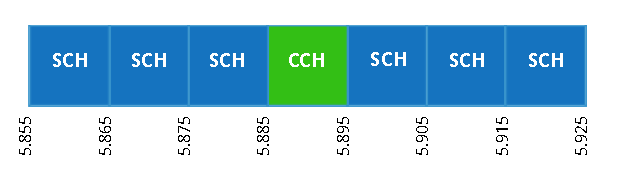
\includegraphics[
        width=0.7\textwidth
    ]{802-11p-spectrum.pdf}
    \caption{Frequency allocation of IEEE 802.11p in the US}
    \label{fig:802-11p-spectrum}
\end{figure}

\begin{enumerate}
    \item SCH1: (5.875 - 5.885 GHz) will be used for safety messages with lower priority (in comparison with CCH) and traffic efficiency applications.
    \item SCH2: (5.895 - 5.905 GHz) will be used for short distance transmissions which results in lower interference for SCH1 and CCH, because of the lower transmit power.
    \item CCH: (5.885 - 5.895 GHz) will be used for high priority safety messages and beacons.
\end{enumerate}
% src: "Characterization of a 5GHz Modular Radio Frontend for WLAN Based on IEEE 802.11p"


% ----- explain higher OSI layers

% IEEE 1609.4 - upper MAC - 
%       Multichannel operation -> 1x Control channel (CCH), 6x Service channel (SCH)

% IEEE 1609.3 - WAVE short message protocol (WSMP)

% IEEE 1609.2 - Security - provides authentication and optional encryption of DSRC messages based on digital signatures and certificates. To protect the privacy of drivers, certificates don’t contain information about the driver. What’s more, a vehicle uses a certificate only for a limited time, changing it frequently to make tracking more difficult.

% Message Dictionary / OSI FACILITY layer
% SAE J2735 - Basic Safety Message (BSM)
%   ~ 300 bits, max. 10Hz
%   beacon messages, vehicle state information
    
% SAE J2945.1 

% Minimal message size              EU          US
% w/ signature & certificate:       186 bit     275 bit
% with signature & certificate      ~2 KBit     ~2 KBit


\begin{figure}[H]
    \centering
    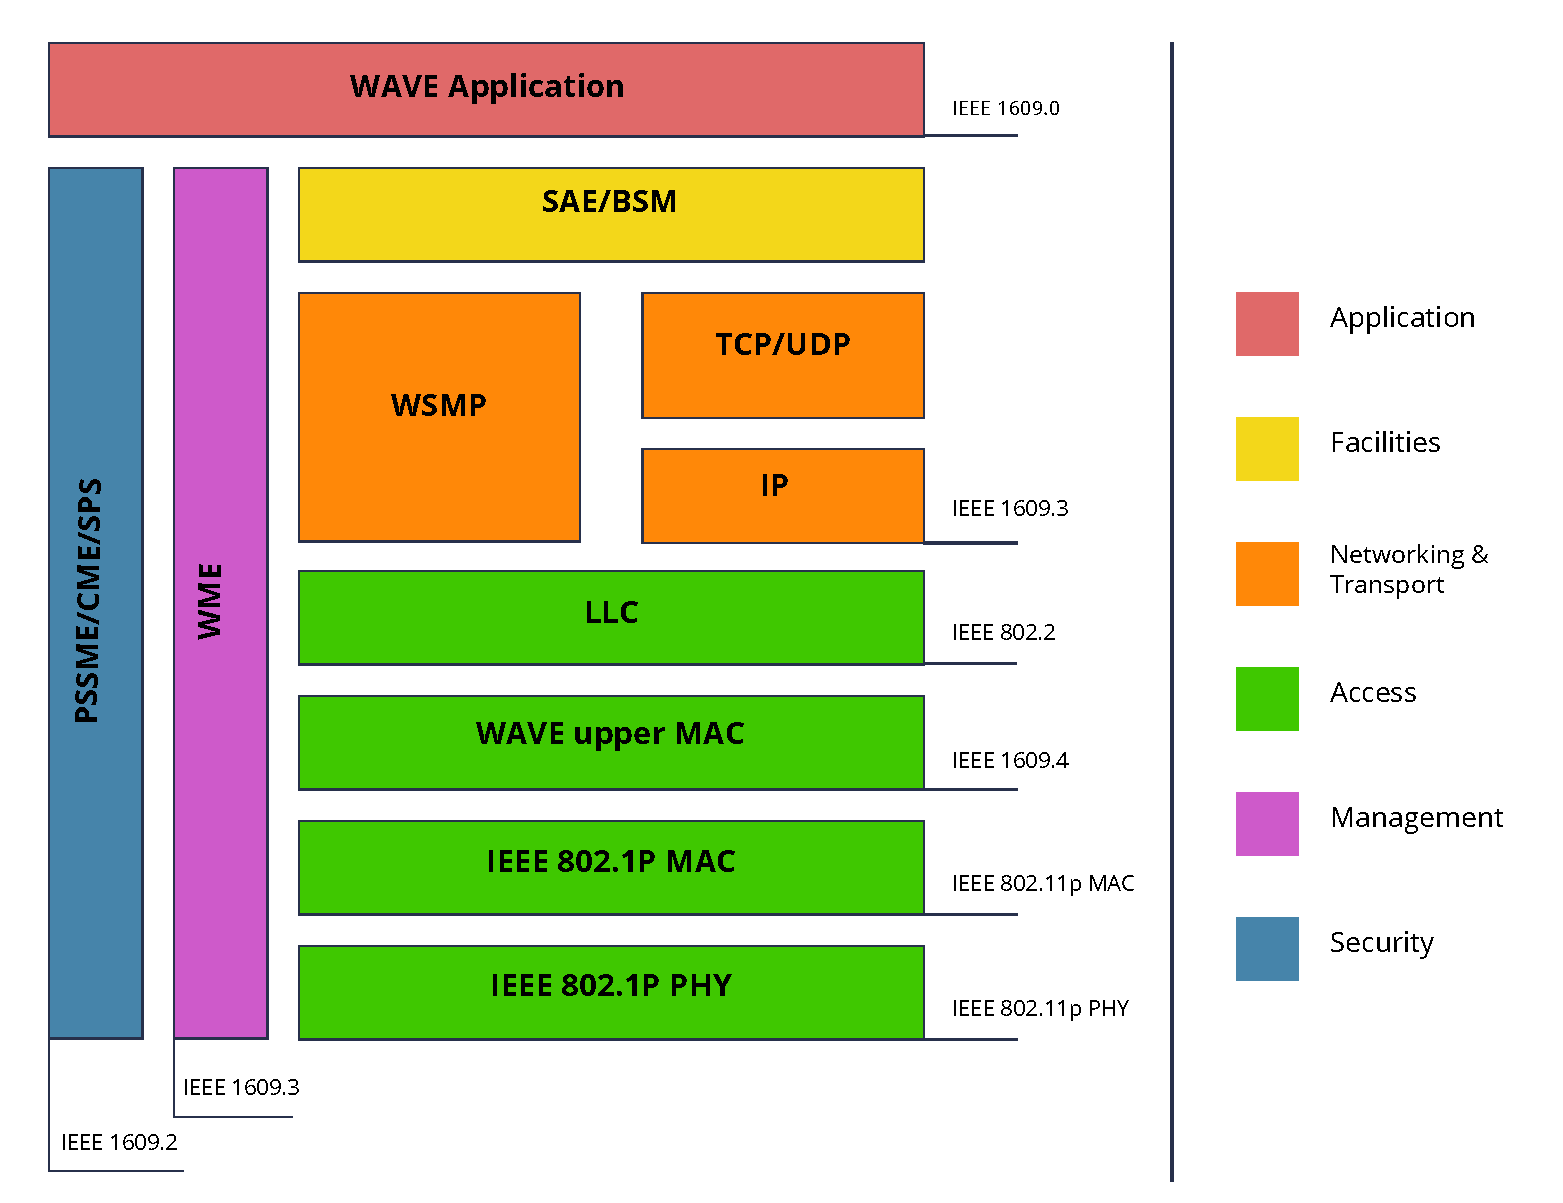
\includegraphics[
        width=\textwidth
    ]{WAVE-IEEE-1609.pdf}
    \caption{WAVE/DSRC procool stack}
    \label{fig:iso-ieee-wave}
\end{figure}


% ----- explain DSRC main goals


% url: http://www.hh.se/download/18.16490bf0133abd6557e8000209/1341267475825/WWVC2011Standardization.KS.pdf
\newpage

\subsection{Cooperative Intelligent Transport Systems (C-ITS)}
% 802.11p for Europe is termed 'ITS-G5' by ETSI, which is derived from IEEE standard.
% ITS-G5 is standardized as ETSI EN 302 663.

% mention similarities/differences of 802.11p and ITS-G5

% ITS-G5
% https://www.etsi.org/deliver/etsi_en/302600_302699/302663/01.02.00_20/en_302663v010200a.pdf

5.725 GHz - 5.875 GHz
% url: https://dsp.stackexchange.com/questions/30300/explaining-communicating-spectra-generating-visualizations


% https://vectr.com/tmp/gRrpW8n57/eDK3uRzv?page=3


% ----- ITS-G5 Channel Freq. spectrum

% ----- [insert ITS-G5 frequency spectrum]

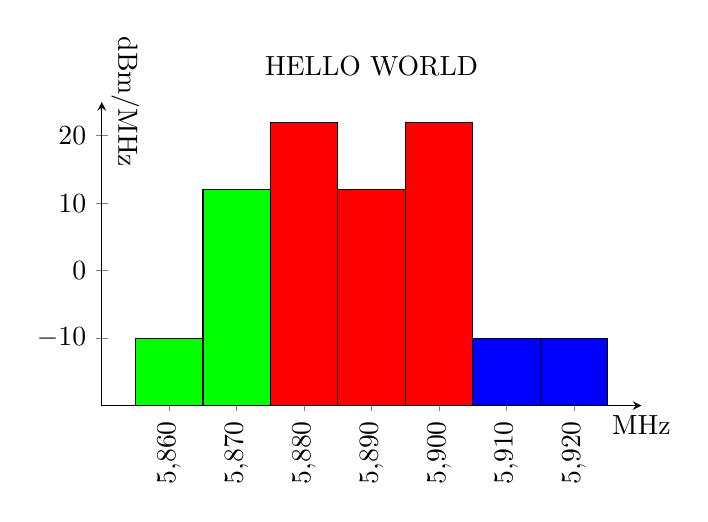
\begin{tikzpicture}
    \centering
    \begin{axis}[
        title=HELLO WORLD,
        xlabel=MHz,
        x label style={at={(axis description cs:1,0)},anchor=north},
        ylabel={dBm/MHz}, %TODO properly
        y label style={
            at={(axis description cs:0,1)},
            anchor=south,
            rotate=180
        },
        xmin=5850, xmax=5930,
        ymin=-20, ymax=25,
        x tick label style={rotate=90},
        xtick={5860, 5870, 5880, 5890, 5900, 5910, 5920},
        ytick={-10, 0, 10, 20},
        axis x line=bottom, axis y line=left,
        axis equal image
        % axis line thick
    ]
    \draw [fill=green]  (axis cs:5855,-20) rectangle (axis cs:5865,-10); %SCH4
    \draw [fill=green]  (axis cs:5865,-20) rectangle (axis cs:5875, 12); %SCH3
    \draw [fill=red]    (axis cs:5875,-20) rectangle (axis cs:5885, 22); %SCH1
    \draw [fill=red]    (axis cs:5885,-20) rectangle (axis cs:5895, 12); %SCH2
    \draw [fill=red]    (axis cs:5895,-20) rectangle (axis cs:5905, 22); %CCH
    \draw [fill=blue]   (axis cs:5905,-20) rectangle (axis cs:5915,-10); %SCH5
    \draw [fill=blue]   (axis cs:5915,-20) rectangle (axis cs:5925,-10); %SCH6
    
    \end{axis}
\end{tikzpicture}


% ITS-G5 A
    % ITS road safety related applications
    % 30 MHz
% ITS-G5 B
    % ITS non-safety application
    % 20 MHz
% ITS-G5 C
    % operations also referred to
    % broadband radio access networks (BRAN),
    % radio local area network (RLAN)
    % and wireless local area network (WLAN)

% ITS-G5 D
    % future ITS applications
    % 

% applies OFDM

% ----- explain higher OSI layers

\begin{figure}[H]
    \centering
    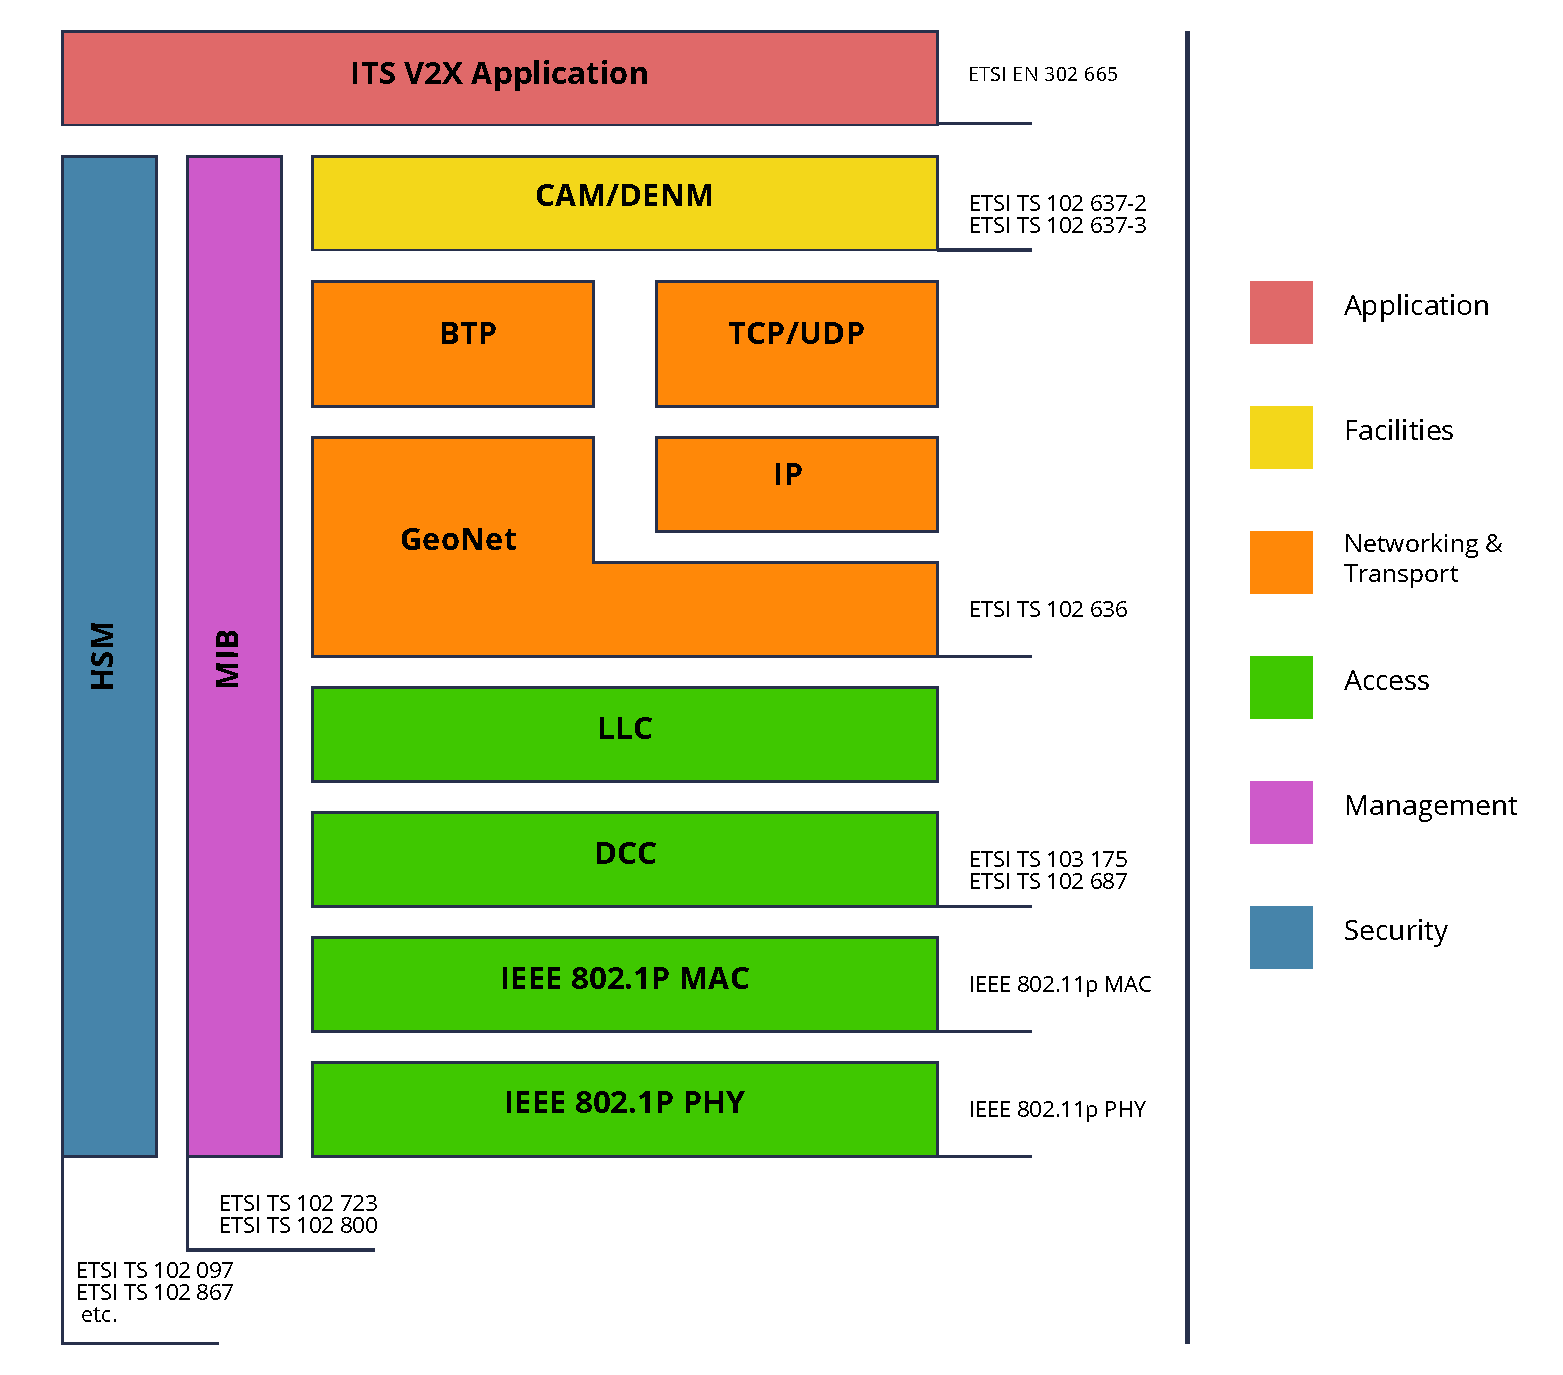
\includegraphics[
        width=\textwidth
    ]{ITS-G5.pdf}
    \caption{meaningful Caption about ITS-G5}
    \label{fig:iso-its-g5}
\end{figure}

% compare EU spectrum with US, (possibly) mention briefly incomparability with Japan


% Message Dictionary / OSI FACILITY layer
% EN 302 637-2 (CAM)
% EN 302 637-3 (DENM)

% mention example application (OSI application)

\subsection{Cellular-V2X (C-V2X)}
% V2X via LTE (or, future: 5G)

% ETSI TS 122 185
% US ????
                    
% https://ec.europa.eu/transport/sites/transport/files/themes/its/doc/c-its-platform-final-report-january-2016.pdf
% TS 122 185 (maybe more)



% Interoperability
% The ITS-G5 technology and the application software stack have been standardised in the European standardisation body ETSI since 2009 under a European standardisation mandate.14 Its standards are openly accessible to assure interoperability
% https://itsg5-ready-to-roll.eu/ITS-G5-FactSheet.pdf

\newpage

\section{V2X Message Sets}
% [TODO] General info, introduction to Message sets


\subsection{Cooperative Awareness Messages (CAM)}
%   ETSI EN 302 637-2

% --- explain cam structure (it's containers and each field)
% use cases, in which applications there used
% generation time

% CAM table

CAM generation frequency: 100 - 1000 ms (or 1-10Hz)
CAM data volume:
    
    Base container
    + HF Container 
    + LF Container
    = ~200 bits
    
    ITS PDU header
    + Signature
    = ~750 bits
    
    certificate = ~1 Kbit

% General structure of a CAM

% ---- [insert example CAM]
\begin{figure}[H]
    \centering
    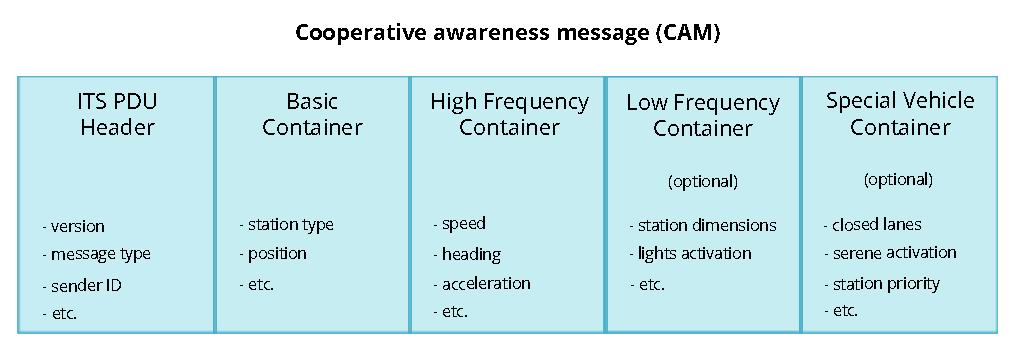
\includegraphics[
        width=\textwidth
    ]{CAM.pdf}
    \caption{Meaningful Caption CAM}
    \label{fig:cam-structure}
\end{figure}


\subsection{Decentralized Environmental Notification Messages (DENM)}
%   ETSI EN 302 637-3

% explain DENM structure....
% its containers
%   each field

% DENM Table
\begin{figure}[H]
    \centering
    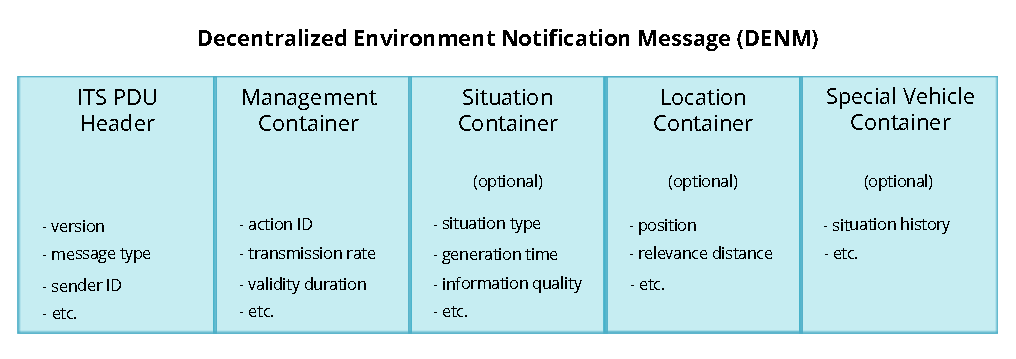
\includegraphics[
        width=\textwidth
    ]{DENM.pdf}
    \caption{meaningful caption DENM}
    \label{fig:denm-structure}
\end{figure}

\chapter{Related Work}
\label{cha:RelatedWork}


\chapter{Concept}
\label{cha:Concept}

\section{Overview}

\section{Kapsch EVK-3300}
\chapter{Implementation}
\label{cha:Implementation}

\section{General Approach}

\section{Architecture}

\section{Entities}

\subsection{Pedestrian}

\subsection{Roadside unit}
% \chapter{Evaluation}
\label{cha:Evaluation}


\chapter{Conclusion}
\label{cha:Conclusion}

\section{Summary}

\section{Future Outlook}


\chapter{Printing the Manuscript}
\label{cha:Printing}



%%%--------------------------------------------------
\appendix           % appendix 
%%%--------------------------------------------------

\chapter{Technical Details}
\label{app:TechnicalDetails}



	% contents of the CD-ROM/DVD

%%%--------------------------------------------------
\MakeBibliography    % references
%%%--------------------------------------------------

%%% special page for checking print size ------------
\chapter*{Check Final Print Size}

\begin{center}
{\Large --- Check final print size! ---}

\bigskip

\calibrationbox{100}{50} % width/height of box in mm

\bigskip

{\Large --- Remove this page after printing! ---}

\end{center}



%%%--------------------------------------------------
\end{document}
%%%--------------------------------------------------